\let\negmedspace\undefined
\let\negthickspace\undefined
\documentclass[journal]{IEEEtran}
\usepackage[a5paper, margin=10mm, onecolumn]{geometry}
%\usepackage{lmodern} % Ensure lmodern is loaded for pdflatex
\usepackage{tfrupee} % Include tfrupee package

\setlength{\headheight}{1cm} % Set the height of the header box
\setlength{\headsep}{0mm}     % Set the distance between the header box and the top of the text

\usepackage{xparse}
\usepackage{gvv-book}
\usepackage{gvv}
\usepackage{cite}
\usepackage{amsmath,amssymb,amsfonts,amsthm}
\usepackage{algorithmic}
\usepackage{graphicx}
\usepackage{textcomp}
\usepackage{xcolor}
\usepackage{txfonts}
\usepackage{listings}
\usepackage{enumitem}
\usepackage{mathtools}
\usepackage{gensymb}
\usepackage{comment}
\usepackage[breaklinks=true]{hyperref}
\usepackage{tkz-euclide} 
\usepackage{listings}
% \usepackage{gvv}                                        
\def\inputGnumericTable{}                                 
\usepackage[latin1]{inputenc}                                
\usepackage{color}                                            
\usepackage{array}                                            
\usepackage{longtable}                                       
\usepackage{calc}                                             
\usepackage{multirow}                                         
\usepackage{hhline}                                           
\usepackage{ifthen}                                           
\usepackage{lscape}
\begin{document}

\bibliographystyle{IEEEtran}
\vspace{3cm}

\title{1.1.8.17}
\author{EE24BTECH11024 - G.Abhimanyu Koushik}
% \maketitle
% \newpage
% \bigskip
{\let\newpage\relax\maketitle}

\renewcommand{\thefigure}{\theenumi}
\renewcommand{\thetable}{\theenumi}
\setlength{\intextsep}{10pt} % Space between text and floats


\numberwithin{equation}{enumi}
\numberwithin{figure}{enumi}
\renewcommand{\thetable}{\theenumi}


\textbf{Question}:\\
The perimeter of triangle with vertices \myvec{0\\4},\myvec{0\\0} and \myvec{3\\0} is
\\
\textbf{Solution: }
\begin{table}[h!]    
  \centering
  \begin{tabular}[12pt]{ |c|c|c|}
    \hline
    \textbf{Symbol} & \textbf{Value} & \textbf{Description} \\
    \hline
    $\vec{A}$ & \myvec{6\\5} & First point\\
    \hline 
    $\vec{B}$ & \myvec{-4\\3} & Second point\\
    \hline
    $\vec{Y}$ & \myvec{0\\$y$} & Point on Y-Axis equidistant from A and B\\
    \hline
    \end{tabular}

  \caption{Variables Used}
  \label{tab10.5.3.9.1}
\end{table}\\
Distance between $\vec{A}$ and $\vec{B}$, $d_1$ is
\begin{align}
	\brak{\vec{A} - \vec{B}} = \myvec{0\\4} - \myvec{3\\0} &= \myvec{-3\\4}\\
	\brak{\vec{A-B}}^\top\brak{\vec{A-B}}&=25\\
    d_1=||\vec{A}-\vec{B}||&=5
\end{align}
Distance between $\vec{A}$ and $\vec{O}$, $d_2$ is
\begin{align}
	\brak{\vec{A} - \vec{O}} = \myvec{0\\4} - \myvec{0\\0} &= \myvec{0\\4}\\
	\brak{\vec{A-O}}^\top\brak{\vec{A-O}}&=16\\
    d_2=||\vec{A}-\vec{O}||&=4
\end{align}
Distance between $\vec{O}$ and $\vec{B}$, $d_3$ is
\begin{align}
	\brak{\vec{O} - \vec{B}} = \myvec{0\\0} - \myvec{3\\0} &= \myvec{-3\\0}\\
	\brak{\vec{O-B}}^\top\brak{\vec{O-B}}&=9\\
    d_3=||\vec{O}-\vec{B}||&=3
\end{align}
Perimeter of the triangle is 
\begin{align}
    d_1+d_2+d_3&=12
\end{align}
\begin{figure}[h!]
   \centering
   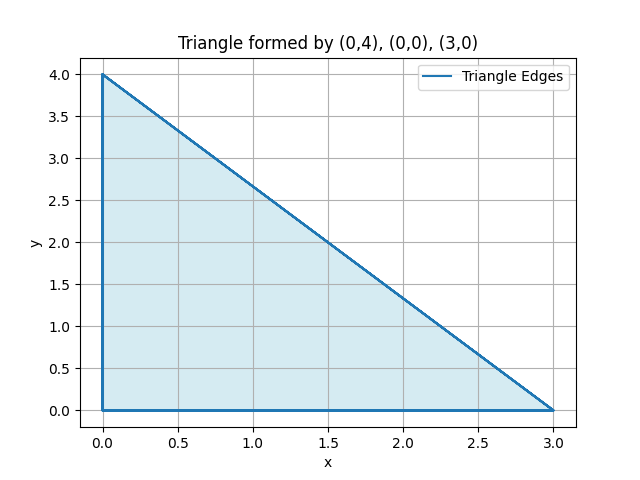
\includegraphics[width=0.7\linewidth]{figs/fig.png}
   \caption{Plot of the triangle}
   \label{stemplot}
\end{figure}
\end{document}  
\end{document}


